\documentclass[a4paper,12pt]{article}
\usepackage[margin=2.2cm]{geometry}
\usepackage{graphicx}
\usepackage{booktabs}
\usepackage{tabularx}
\usepackage{array}
\usepackage{hyperref}
\usepackage{xcolor}
\usepackage{float}
\usepackage{listings}
\usepackage{seqsplit}
\hypersetup{colorlinks=true,linkcolor=blue,urlcolor=blue}
\lstset{basicstyle=\ttfamily\small,breaklines=true,frame=single}
\emergencystretch=3em
\title{Experiment 1: Object Detection and Recognition}
\author{Student: \underline{\hspace{4cm}}\\ Student ID: \underline{\hspace{4cm}}}
\date{August 2026}
\begin{document}
\maketitle

\begin{abstract}
This experiment develops and deploys a four-class desktop-object detector for mouse, laptop, cup, and phone. Images were collected from videos, annotated in ISAT, converted to YOLO format, and used to fine-tune YOLOv8n. The final checkpoint was executed on a Jetson Orin with a USB camera. On a correlated temporal-frame diagnostic set, the detector matched 103 of 104 annotated objects, giving 100.00\% precision and 99.04\% recall. A representative Jetson frame displayed simultaneous detections and 15.0 FPS. These results demonstrate a working prototype, while the required independent 20-object accuracy test, stable averaged FPS log, and end-to-end ROS2 runtime record must still be completed before the results can be claimed as final course acceptance.
\end{abstract}

\section{Objective and Acceptance Criteria}
The objectives were to (1) detect at least two types of desktop objects, (2) train a detector using self-collected and annotated data, (3) run the detector on Jetson, (4) display class, bounding box, confidence, and frame rate in real time, and (5) publish detection results through ROS2. The course acceptance criteria require at least two simultaneously recognizable classes, testing on at least 20 objects with accuracy no lower than 80\%, Jetson speed of at least 5 FPS, and preservation of result videos and typical error cases.

\section{Hardware and Software}
\begin{table}[H]\centering\caption{Experimental environment}\begin{tabularx}{\textwidth}{lX}
\toprule Item & Configuration \\
\midrule
Training computer & Windows 11; NVIDIA GPU and CUDA details should be filled from the training machine.\\
Embedded computer & Jetson Orin, aarch64, Ubuntu 20.04.6, L4T R35.6.4 / JetPack 5.1.6.\\
GPU software & CUDA 11.4; NVIDIA PyTorch 2.0.0a0; torchvision 0.15.1 with working CUDA NMS.\\
Python and framework & Python 3.8 on Jetson; Ultralytics 8.4.22; YOLOv8n.\\
Camera & USB camera at 640$\times$480 input; exact model: \underline{\hspace{3cm}}.\\
ROS2 & `rclpy`, `cv\_bridge`, `sensor\_msgs`, and `vision\_msgs`; distribution: \underline{\hspace{2cm}}.\\
\bottomrule\end{tabularx}\end{table}

\section{Dataset and Annotation}
The dataset contains 595 images from self-recorded videos. The four classes are \texttt{mouse}, \texttt{laptop}, \texttt{cup}, and \texttt{phone}. ISAT polygon annotations were converted to YOLO bounding boxes. The conversion script recomputes each box from the polygon, validates normalized coordinates, removes near-duplicate boxes, and records provenance in a manifest.

\begin{table}[H]\centering\caption{Dataset split and object counts}\begin{tabular}{lrrr}
\toprule Split & Images & Objects & Objects per class (mouse/laptop/cup/phone)\\
\midrule Train & 421 & 506 & 119/85/212/90\\
Validation & 87 & 104 & 28/17/42/17\\
Test diagnostic & 87 & 104 & 28/17/42/17\\
\bottomrule\end{tabular}\end{table}

The split uses contiguous temporal blocks within each of 19 source groups. This prevents random frame shuffling, but the same physical source groups occur in all three splits. Therefore, neighboring-frame correlation remains and the diagnostic set is not an independent physical-object benchmark.

\section{Method}
The COCO-pretrained YOLOv8n model was fine-tuned as a four-class detector. Training used 100 epochs, 640-pixel input images, batch size 16, GPU device 0, zero data-loader workers, deterministic seed 42, automatic optimizer selection, standard YOLO data augmentation, and early-stopping patience of 25. Training used only the train and validation splits; the diagnostic test split was not used for optimization.

\begin{lstlisting}[caption={Reproduction command}]
python train_yolo.py --epochs 100 --batch 16 --device 0 --workers 0
\end{lstlisting}

\section{Training and Frame-Level Diagnostic Results}
The best recorded validation mAP@0.5:0.95 was 0.98571 at epoch 76. At epoch 100, precision was 0.99417, recall was 0.99405, mAP@0.5 was 0.99104, and mAP@0.5:0.95 was 0.98078. The complete curves and confusion matrices are stored in \path{training/yolov8n_4class_finetune/}.

\begin{figure}[H]\centering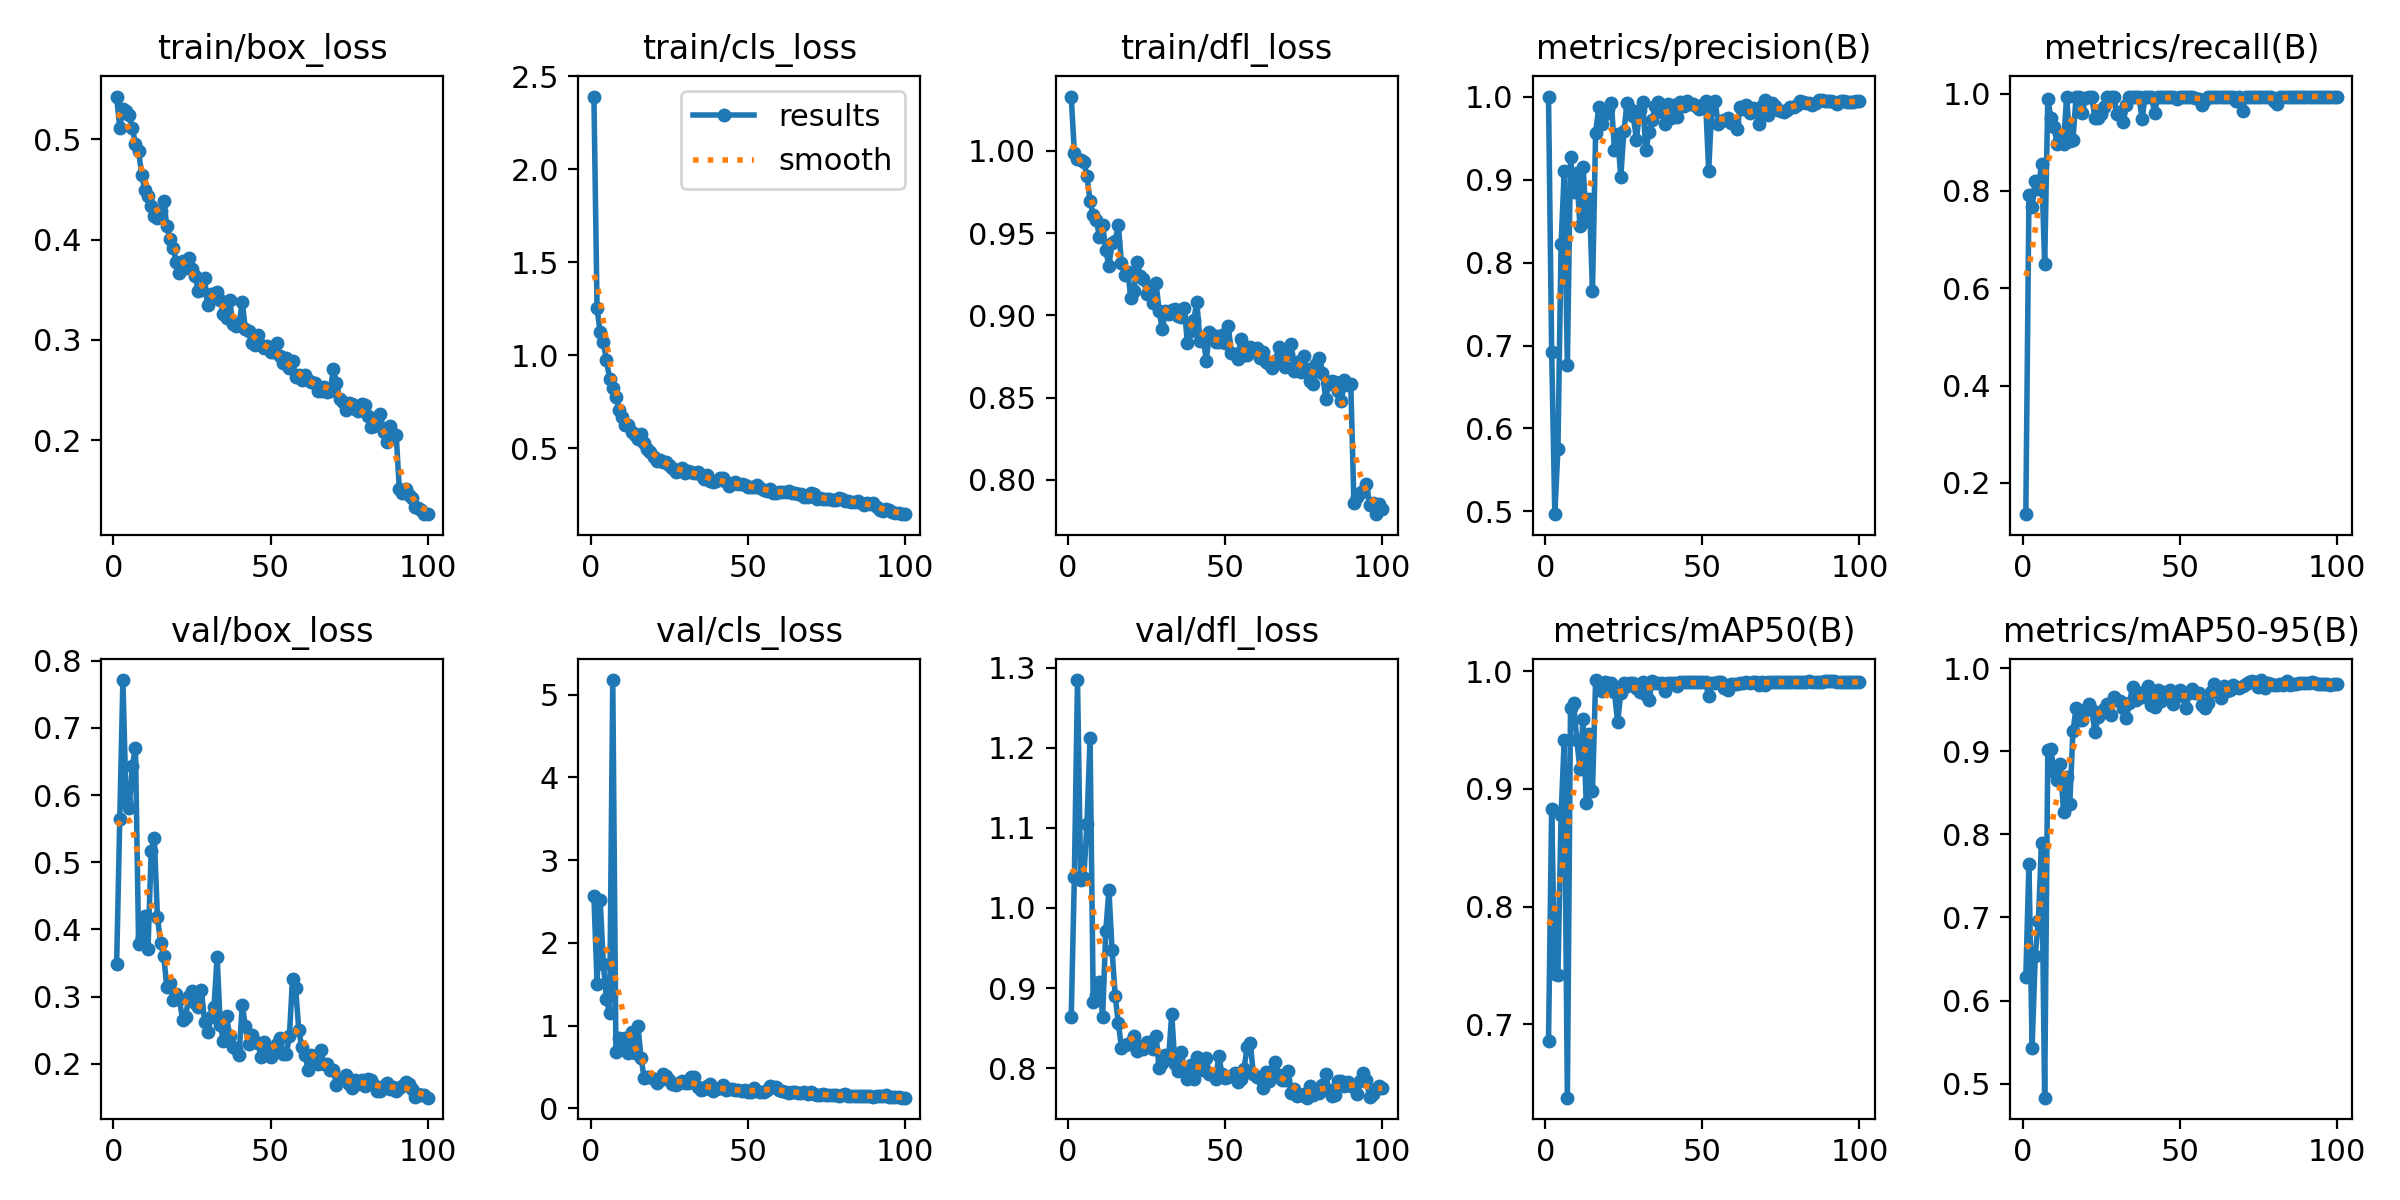
\includegraphics[width=0.98\textwidth]{../training/yolov8n_4class_finetune/results.png}\caption{Training losses and validation metrics over 100 epochs. The curves show convergence and late-stage stabilization. Because only one run is available, run-to-run variation cannot be estimated.}\label{fig:training}\end{figure}

At confidence threshold 0.25 and matching IoU threshold 0.50, 103 of 104 annotated objects were matched. There was one false negative and no false positives.

\begin{table}[H]\centering\caption{Frame-level diagnostic by class}\begin{tabular}{lrrrr}\toprule Class & Ground truth & Correct & FN & Recall \\\midrule
Mouse & 28 & 28 & 0 & 100.00\%\\
Laptop & 17 & 17 & 0 & 100.00\%\\
Cup & 42 & 41 & 1 & 97.62\%\\
Phone & 17 & 17 & 0 & 100.00\%\\
\midrule Total & 104 & 103 & 1 & 99.04\%\\\bottomrule\end{tabular}\end{table}

\begin{figure}[H]\centering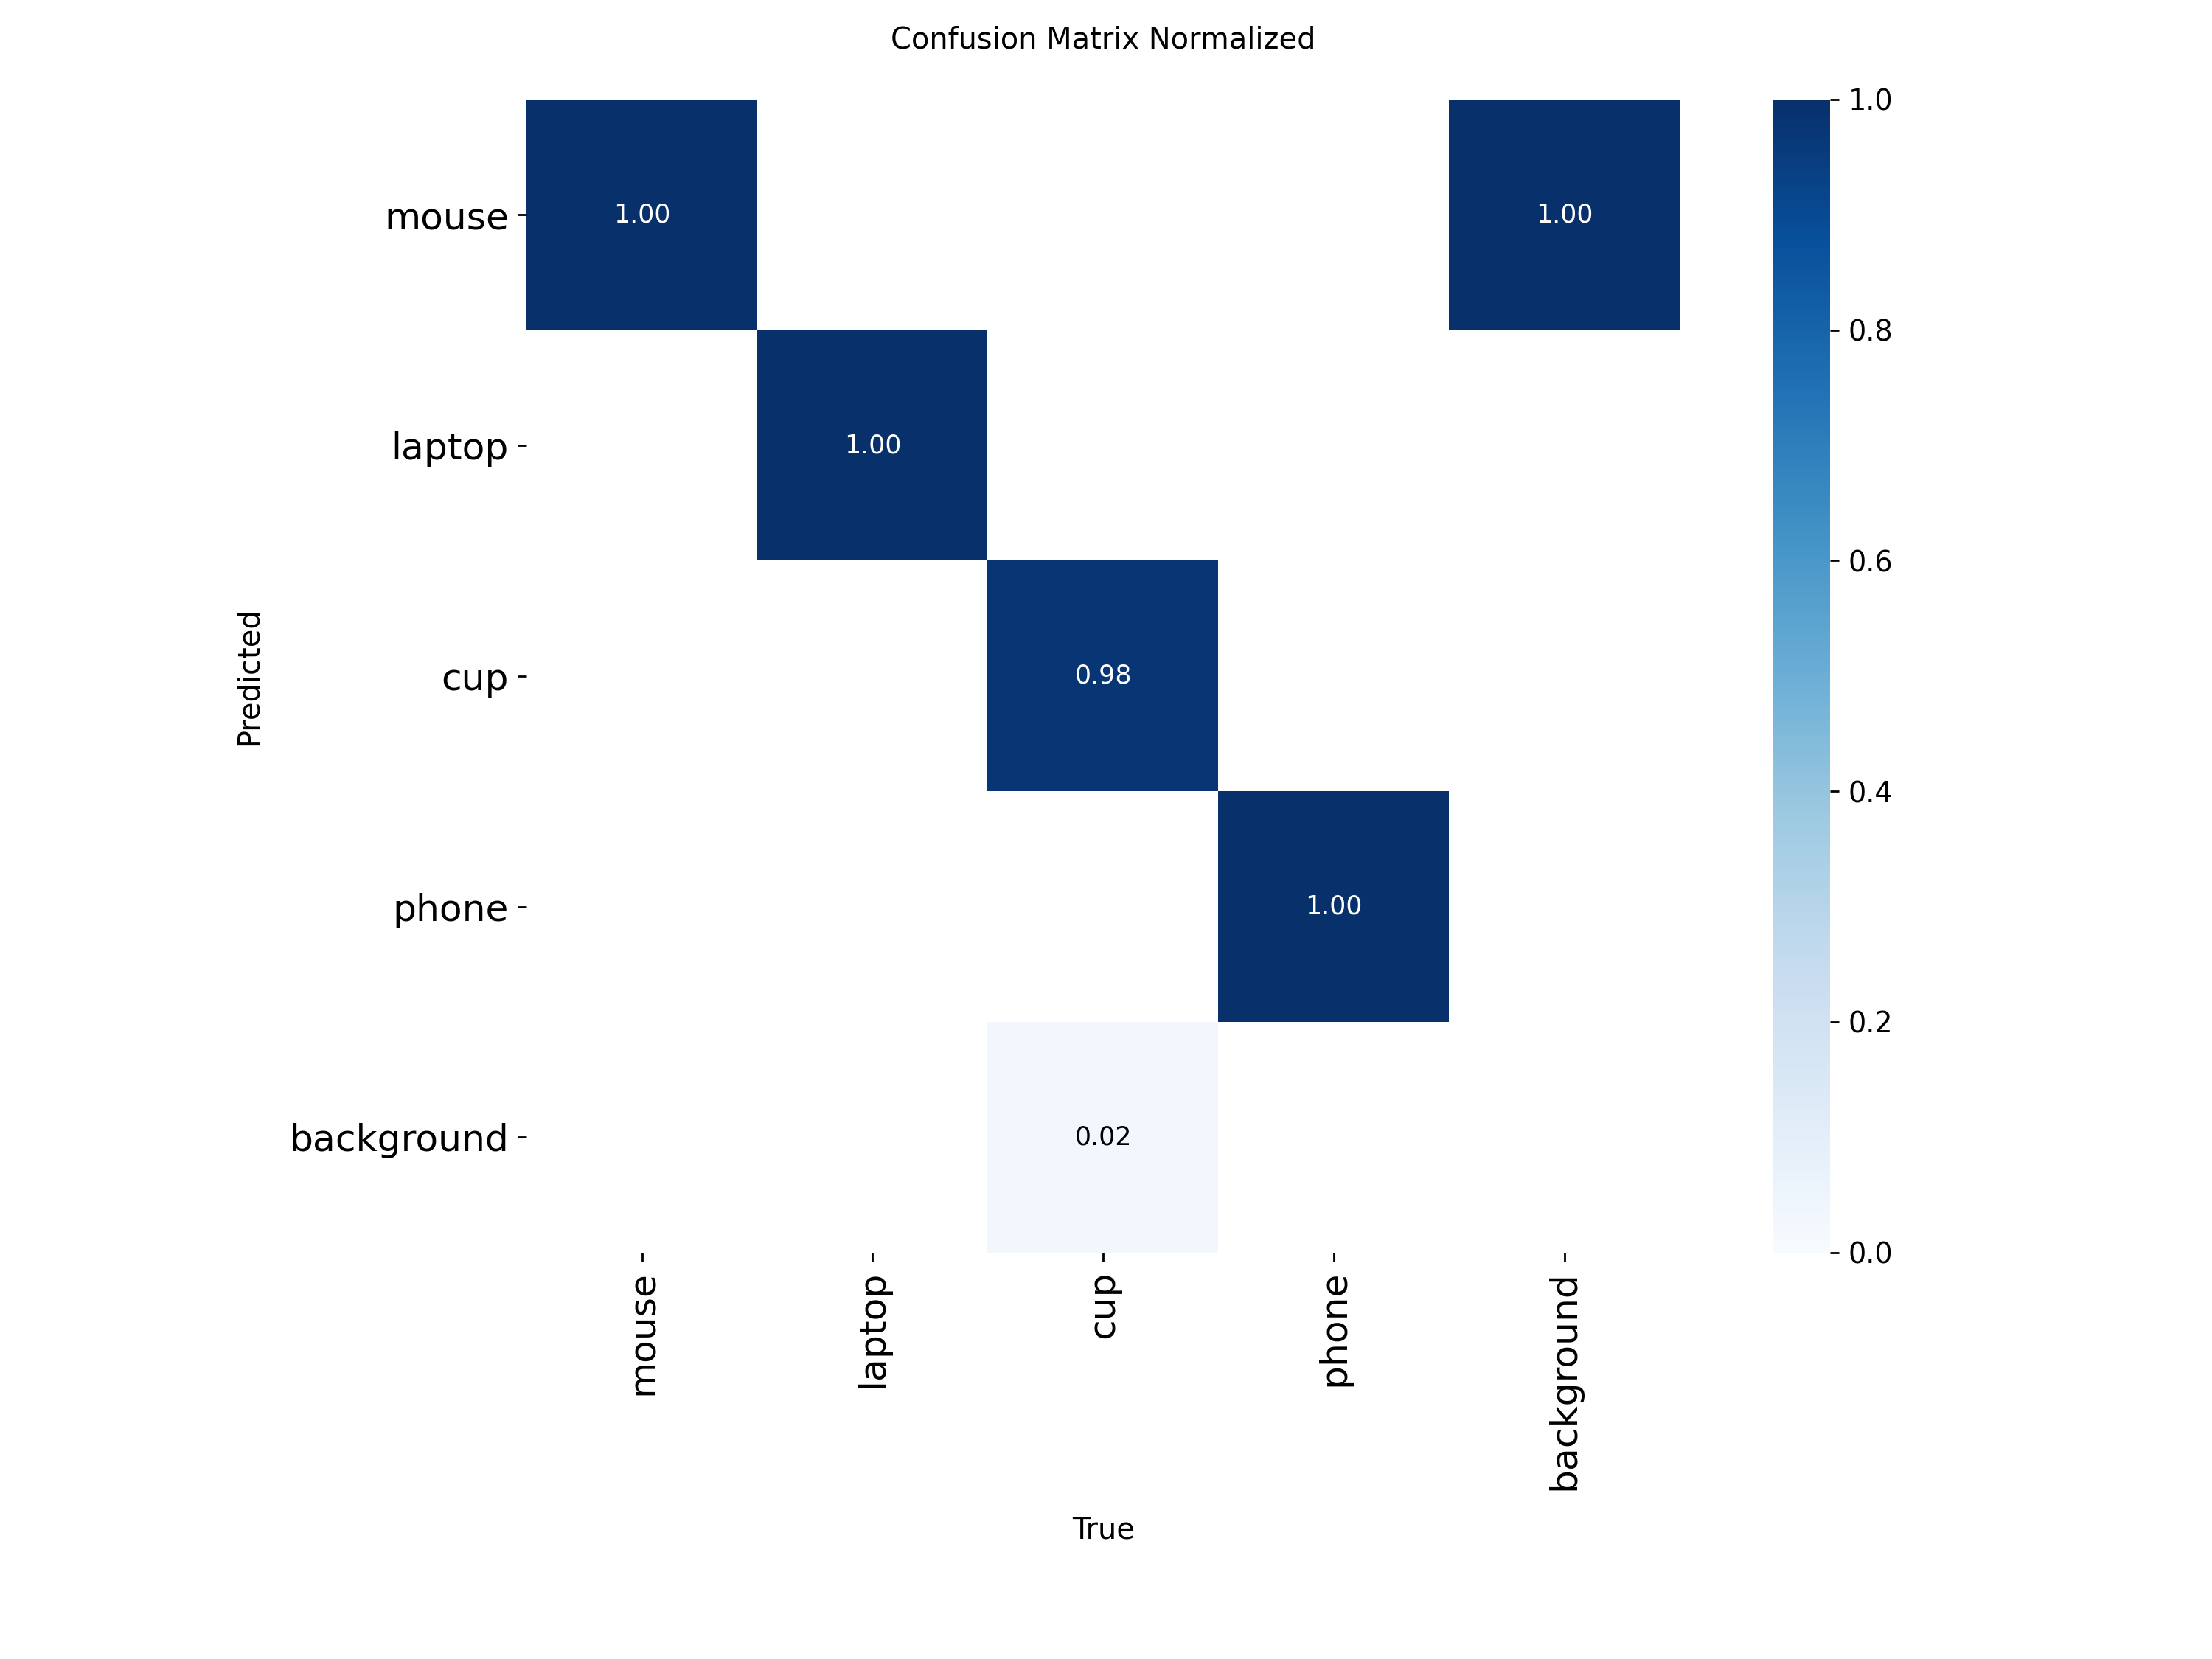
\includegraphics[width=0.75\textwidth]{../training/yolov8n_4class_finetune/confusion_matrix_normalized.png}\caption{Normalized validation confusion matrix. The dominant diagonal indicates that class confusion was limited on the validation frames.}\label{fig:cm}\end{figure}

The 99.04\% value is a frame-level diagnostic result only. It must not be reported as the final real-world accuracy because temporal frames from related source groups occur in both training and testing.

\section{Jetson Deployment and Real-Time Detection}
The checkpoint \texttt{weights/best.pt} was copied to Jetson and loaded by \texttt{realtime\_detect.py}. The program uses V4L2 for a USB camera, performs GPU inference, draws bounding boxes and confidence scores, counts objects by class, calculates a sliding-window FPS, and optionally writes an annotated MP4 file.

\begin{lstlisting}[caption={Jetson real-time command}]
python realtime_detect.py --weights ~/robotics_exp1/weights/best.pt \\
  --source 0 --imgsz 320 --confidence 0.35 --device 0 \\
  --camera-width 640 --camera-height 480 --camera-fps 30 \\
  --output ~/robotics_exp1/results/demo.mp4
\end{lstlisting}

\begin{figure}[H]\centering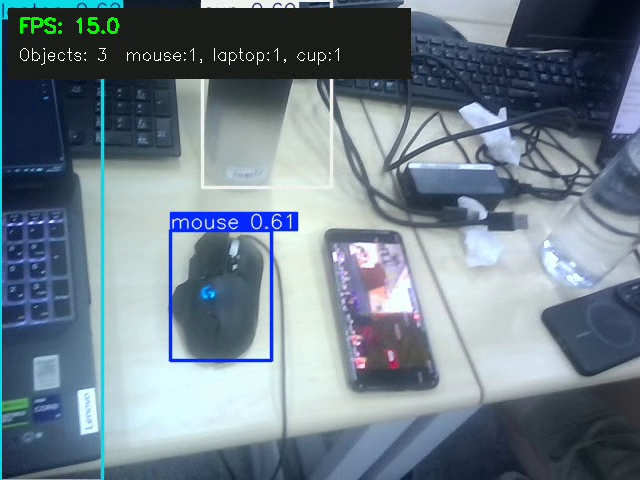
\includegraphics[width=0.9\textwidth]{figures/jetson_demo_frame.jpg}\caption{Representative Jetson demo frame. The overlay shows simultaneous mouse, laptop, and cup detections, confidence scores, object counts, and a displayed FPS of 15.0. This is an observed sliding-window value, not a saved time-averaged benchmark.}\label{fig:jetson}\end{figure}

The saved demonstration video is \texttt{results/jetson\_demo.mp4}. The final report should add the measured mean and minimum FPS over a continuous 30--60 second run. Required field: \textbf{mean FPS = \underline{\hspace{2cm}}; minimum FPS = \underline{\hspace{2cm}}; pass (mean $\geq$ 5 FPS): \underline{\hspace{1.5cm}}}.

\section{ROS2 Publication}
The node \texttt{ros2\_detector\_node.py} subscribes to \texttt{/camera/image\_raw} as \texttt{sensor\_msgs/Image}. It converts images with \texttt{cv\_bridge}, performs YOLO inference, and publishes \texttt{vision\_msgs/Detection2DArray} on \texttt{/detections}. Each detection contains a pixel-coordinate center, width, height, class name, and confidence score.

\begin{lstlisting}[caption={ROS2 verification command}]
python ros2_detector_node.py --weights ~/robotics_exp1/weights/best.pt \\
  --image-topic /camera/image_raw --output-topic /detections --device 0
ros2 topic echo /detections --once
\end{lstlisting}

The implementation is present, but an end-to-end runtime capture has not yet been archived. Insert the terminal screenshot or bag/topic record here: \textbf{ROS2 evidence: \underline{\hspace{7cm}}}.

\section{Independent 20-Object Test}
The course accuracy requirement must be measured on at least 20 distinct physical objects that were not merely adjacent video frames. Record one row per object in \texttt{results/independent\_test\_template.csv}.

\begin{table}[H]\centering\caption{Independent acceptance test (to be completed)}\begin{tabular}{lrrr}\toprule Class & Tested & Correct & Accuracy \\\midrule Mouse & \underline{\hspace{1cm}} & \underline{\hspace{1cm}} & \underline{\hspace{1cm}}\\ Laptop & \underline{\hspace{1cm}} & \underline{\hspace{1cm}} & \underline{\hspace{1cm}}\\ Cup & \underline{\hspace{1cm}} & \underline{\hspace{1cm}} & \underline{\hspace{1cm}}\\ Phone & \underline{\hspace{1cm}} & \underline{\hspace{1cm}} & \underline{\hspace{1cm}}\\\midrule Total & \underline{\hspace{1cm}} & \underline{\hspace{1cm}} & \underline{\hspace{1cm}}\\\bottomrule\end{tabular}\end{table}

Accuracy is calculated as $100\times$ correctly recognized objects divided by tested objects. For exactly 20 objects, at least 16 correct predictions are needed to meet 80\%.

\section{Typical Error Cases and Discussion}
The saved error image \path{results/yolov8n_4class_finetune_test/errors/cup_cup4_000086.jpg} records the only missed object in the frame diagnostic. Cups can be difficult because reflective surfaces, changing viewpoints, partial occlusion, and visually similar backgrounds weaken appearance cues. Practical improvements include collecting more viewpoints and lighting conditions, adding background diversity, balancing source groups, checking annotation consistency, and tuning the confidence threshold on an independent validation set.

\section{Conclusion}
This experiment produced a deployable YOLOv8n detector for four desktop-object classes and demonstrated Jetson-side real-time visualization with an observed 15.0 FPS overlay. The saved frame-level diagnostic reached 103/104 matched objects (99.04\% recall/object accuracy), with one cup miss. The code also implements ROS2 publication and result-video saving. The strongest supported conclusion is that the prototype is operational; final course acceptance must be confirmed by inserting the independent 20-object accuracy table, a stable averaged FPS measurement, and ROS2 topic evidence. No claim of final independent accuracy is made before those measurements are completed.

\section*{Reproducibility Index}
\begin{itemize}
\item Dataset configuration: \path{dataset/yolo/data.yaml}; conversion summary: \path{dataset/yolo/conversion_summary.json}.
\item Final checkpoint: \path{weights/best.pt}; SHA-256: \texttt{\seqsplit{595C8FD32BE2A733BF0845A5FC89847DAD425A1FDEC249C0375E0DEA9B9CFBA5}}.
\item Training metrics: \path{training/yolov8n_4class_finetune/results.csv} and plots.
\item Evaluation: \path{results/yolov8n_4class_finetune_test/summary.json} and \path{per_image.csv}.
\item Deployment and ROS2 source: \path{jetson_setup/deploy_to_jetson.ps1}, \path{realtime_detect.py}, and \path{ros2_detector_node.py}.
\item Demonstration video: \texttt{results/jetson\_demo.mp4}.
\end{itemize}
\end{document}
